\section{Theorie}
\label{sec:Theorie}
Um die Dipolrelaxation in einem Ionenkristall zu charakterisieren, müssen die spezifische Aktivierungsenergie $W$ sowie die Relaxationszeit $\tau_\mathrm{0}$ bestimmt werden, in diesem Abschnitt wird darauf im Folgenden näher
eingegangen.
\subsection{Dipole in Ionenkristallen}
\label{sec:11}
Ein Ionenkristall ist nach außen neutral geladen, dies liegt daran, dass im Inneren abwechselnd negativ und positiv geladene Ionen vorhanden sind. Durch Dotierung derartiger Kristalle mit doppelt geladenen Ionen ist es möglich, dass ein
Dipol entsteht. Dies geschieht dadurch, dass um die Ladungsneutralität nach außen zu erhalten Kationen-Leerstellen im Kristall entstehen. In Abbildung (\ref{fig:doti}) ist dies schematisch dargestellt.
\begin{figure}[h!]
  \centering
  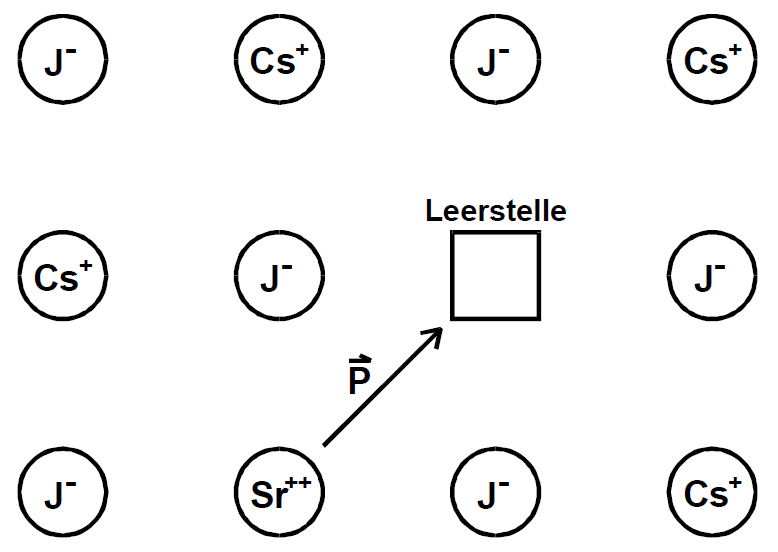
\includegraphics[scale=0.5]{fig/Dipol.png}
  \caption{Dipolbildung innerhalb eines Cäsiumkristalls.}
  \label{fig:doti}
\end{figure}
Wie in Abbildung (\ref{fig:doti}) zu sehen, wird in diesem Beispiel ein zweifach geladenes Strontium genutzt um die Leerstelle zu bilden, dabei ist $\vec{P}$ das Dipolmoment. Der Abstand zwischen Ion und Leerstelle gibt somit
die Richtung des Dipols an. Daraus folgt, dasss aufgrund der Gitterstruktur nur bestimmte Dipolrichtungen im Kristall erlaubt sind. \\ Eine Richtungsänderung der Dipole zu erzwingen ist für $T<\SI{500}{\degreeCelsius}$ nur per Leerstellendiffusion möglich. Diese tritt bei der spezifischen Aktivierungsenergie $W$ auf. Auf diese wird in Abschnitt (\ref{sec:akti}) näher eingegangen. Mithilfe der Boltzmannstatistik, die den Anteil der Dipole angibt, der die nötige
Energie aufbringen kann, ist es nun möglich eine Gleichung für die Relaxationszeit eines Dipols anzugeben:
\begin{equation}
  \label{eqn:relax}
  \tau(T)=\tau_\mathrm{0}\exp\left(\dfrac{W}{k_\mathrm{B}T}\right)
\end{equation}
Dabei ist $\tau_\mathrm{0}$ die charakteristische Relaxationszeit, also der Wert für $T\rightarrow\infty$, $k_\mathrm{B}$ ist die Boltzmannkonstante, diese ist gegeben durch $k_\mathrm{B}=\SI{1.380649e-23}{\joule\per\kelvin}$ \cite{Anleitung7}.
\subsection{Messverfahren}
\label{sec:messv}
In diesem Abschnitt wird der Messvorgang näher beschrieben und die darausfolgenden Berechnungen vorgestellt. Die verwendete Probe fungiert als Dielektrikum in einem Plattenkondensator und hat in etwa eine Dicke von $d=\SIrange{3}{5}{\milli\meter}$. Zunächst wird die Probe polarisiert, dies geschieht durch das Anlegen eines elektrischen Feldes $E$ über einen Zeitraum der wesentlich größer als die Relaxationszeit ist, also $t_\mathrm{pol}\gg\tau(T)$.
Der Anteil der Dipole $\gamma$ der in Feldrichtung weist, kann für $pE\ll k_\mathrm{B}T$ wie folgt genähert werden:
\begin{equation}
  \label{eqn:anteil}
  \gamma(T)=\dfrac{pE}{3k_\mathrm{B}T}
\end{equation}
Nun wird die Probe mithilfe von flüssigem Stickstoff auf eine Temperatur $T_\mathrm{0}$ abgekühlt. Durch Kurzschließen des Kondensators kann die verbleibende Ladung abfließen,
anschließend wird die Probe mit konstanter Heizrate $a$ erhitzt.
\begin{equation}
  a\coloneqq\dfrac{\mathrm{d} T}{\mathrm{d} t}= \mathrm{const.}
\end{equation}
Der Relaxationsvorgang beginnt, das statistische Gleichgewicht stellt sich langsam ein. Ein Depolarisationsstrom $I(T)$ wird dadurch induziert.
Dieser wird wie folgt beschrieben:
\begin{equation}
  \label{eqn:stromdichte}
  I(T)=\gamma(T_\mathrm{p})p\dfrac{\mathrm{d} N}{\mathrm{d} t}
\end{equation}
Dabei gibt $\gamma(T_\mathrm{p})$ den Anteil der Dipole an bei der Polarisationstemperatur $T_\mathrm{0}$ an, der Differenzquotient $\dfrac{\mathrm{d} N}{\mathrm{d} t}$ gibt die Anzahl der pro Zeit und Volumen relaxierenden Dipole an und
$p$ das Dipolmoment. In Abbildung (\ref{fig:stromdi}) ist der Verlauf des Polarisationsstrom dargestellt.
\begin{figure}[h!]
  \centering
  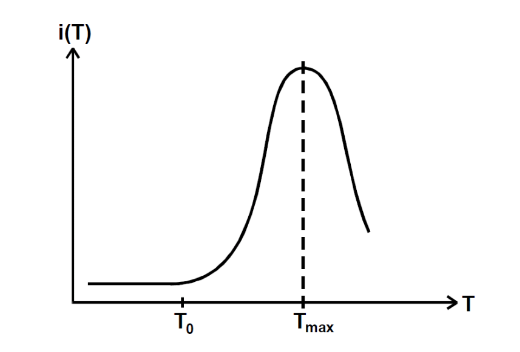
\includegraphics[scale=0.5]{fig/stromver.png}
  \caption{Der Polarisationsstrom aufgetragen gegen die Temperatur.}
  \label{fig:stromdi}
\end{figure}
Mit Gleichung (\ref{eqn:anteil}) lässt sich der erste Teil Gleichung für den Strom wie folgt ausdrücken:
\begin{equation}
  \label{eqn:stromdi2}
  \gamma(T_\mathrm{p})p=\dfrac{p^2E}{3 k_\mathrm{b} T_\mathrm{P}}
\end{equation}
Betrachtet man nun den Differenzquotienten $\dfrac{\mathrm{d} N}{\mathrm{d} t}$ so ist dieser proportional zu $N$ mit dem Faktor $\dfrac{1}{\tau}$. Über Integration lässt sich $N$ bestimmen:
\begin{align}
  \dfrac{\mathrm{d} N}{\mathrm{d} t}&=-\dfrac{N}{\tau(T)} \notag \\
  \label{eqn:einset}
  \Leftrightarrow N&=N_\mathrm{0}\exp\left(-\dfrac{1}{a}\int_{T_0}^T\dfrac{\mathrm{d} T'}{\tau(T')}\right)
\end{align}
Dabei gibt $N_\mathrm{0}$ die Anzahl der Dipole pro Volumeneinheit die beim Beginn des Heizvorgangs bereits orientiert sind. Setzt man dies in Gleichung (\ref{eqn:stromdi}) ein ergibt sich insgesamt für den Strom $I(T)$:
\begin{equation}
  \label{eqn:stromdi3}
  I(T) = \dfrac{p^2 E}{3k_\mathrm{B}T_\mathrm{P}}\dfrac{N_\mathrm{0}}{\tau_\mathrm{0}} \exp{\left(-\dfrac{1}{a\tau_\mathrm{0}}\int_{T_0}^T\exp{\left(-\dfrac{W}{k_\mathrm{B}T'}\right)\mathrm{d}T'}\right)}\exp{\left(-\dfrac{W}{ k_\mathrm{B}T}\right)}
\end{equation}
\subsection{Aktivierungsenergie}
\label{sec:akti}
In diesem Abschnitt werden zwei Verfahren zur Berechnung der Aktivierungsenergie $W$ vorgestellt.
\subsubsection{Polarisationsansatz}
Es wird angenommen, dass die Aktivierungsenergie $W$ groß im Vergleich zur thermischen Energie $k_\mathrm{b} T$ ist. Für eine kleine Temperaturdifferenz $T-T_\mathrm{0}$ wird das Integral in Gleichung (\ref{eqn:stromdi3}) zu:
\begin{align*}
  \int_{T_0}^T\exp{\left(-\dfrac{W}{k_\mathrm{B}T'}\right)\mathrm{d}T'}\approx0
\end{align*}
Damit folgt für den Strom $I(T)$:
\begin{equation}
  \label{eqn:polarime}
  I(T)\approx \dfrac{p^2 E}{3k_\mathrm{B}T_\mathrm{P}}\dfrac{N_\mathrm{0}}{\tau_\mathrm{0}}\exp\left(-\dfrac{W}{k_\mathrm{B}T}\right)
\end{equation}
Durch eine halblogarithmische Darstellung kann nun die Aktivierungsenergie $W$ ermittelt werden.
\subsubsection{Herleitung über die Stromdichte}
